\subsection*{Fase 5: Minería de datos}
En esta etapa se utilizo el algoritmo \textit{k-means}, el cual hace parte del tipo de aprendizaje no supervisado, y es una de las técnicas de clustering \footnote{agrupamiento} más utilizada por su sencillez y rapidez. En este modelo, se dividen los datos en \textit{k-clusters} asignando cada objeto a su centroide de cluster más cercano (el valor medio de las variables para todos los objetos en ese cluster en particular) basado en la medida de la distancia utilizada. Es más robusto ante diferentes tipos de variables. Además, es rápido para grandes conjuntos de datos, que son habituales en la segmentación \cite{Dean2014}. El algoritmo \textit{k-means} presenta los siguientes pasos:

\begin{enumerate}
	\item Elegir el número de \textit{k-clusters}.
	\item Seleccionar \textit{k-centros} del clúster. Para ello, se debe elegir al azar \textit{k} objetos del conjunto de datos.
	\item Asignar cada objeto al centroide de cluster más cercano.
	\item Re-calcular el nuevo centroide del clúster.
	\item Repetir los pasos 3 y 4 hasta que se cumpla el criterio de convergencia o se alcance la máxima iteración.
\end{enumerate}

Cabe resaltar, que este algoritmo fue seleccionado en función de los objetivos particulares definidos en la fase 1. Para ejecutarlo, se utilizo el lenguaje multi-paradigma \textit{Python} debido a la gran cantidad librerías que permiten agilizar el entrenamiento de algoritmos de aprendizaje no supervisado. En este caso se realizó un análisis con base al agrupamiento de la totalidad de datos conformado por $8481$ filas y $6$ columnas. 

\begin{figure}[h!]
	\centering
	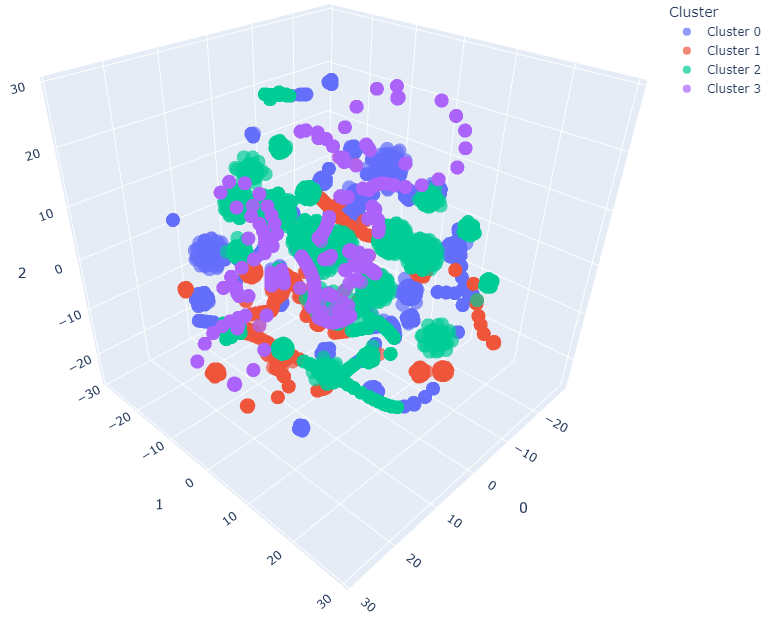
\includegraphics[width=1
	\linewidth]{IMAGENES/Tsne}
	\caption{Gráfica T-SNE para clusters.}
	\label{TSNE}
\end{figure} 

A continuación se le asigno a la creación del modelo una tolerancia del $0.0001$ con la cual le tomo un máximo de 300 iteraciones para obtener un totalidad de 4 clusters. El resultado puede ser observado en la figura \ref{TSNE}, la cual fue generada con el método T-SNE \footnote{T-distributed Stochastic Neighbor Embedding}, el cual permite generar una distribución de probabilidad que representa las similitudes entre vecinos en un espacio de gran dimensión y en un espacio de menor dimensión. Para un mejor entendimiento del resultado obtenido, en la figura \ref{Distance} se observa la distancia entre clusters con respecto a la posición inicial generada por el modelo.

\begin{figure}[h!]
	\centering
	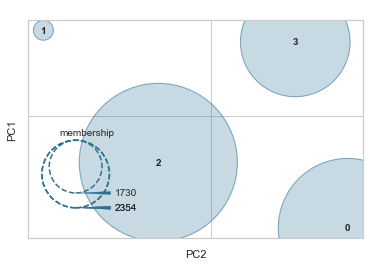
\includegraphics[width=1
	\linewidth]{IMAGENES/Distance}
	\caption{Mapas de distancia entre clusters.}
	\label{Distance}
\end{figure} 

Cabe resaltar, que para la creación, entrenamiento y prueba del modelo se utilizo una maquina equipada con un procesador Intel Core i7-11370H de 11th generación con una frecuencia de 3.30 GHz-4.9 GHz , una tarjeta NVIDIA GeForce RTX 3050, un disco duro SSD Samsung con una velocidad de lectura de  7,000 MB/s y 48GB de memoria RAM. 

Simultáneamente para demostrar el comportamiento predictivo del modelo se utilizo el $95\%$ de los datos para el entrenamiento y el $5\%$ de datos restante para comprobar la precisión en la predicción del agrupamiento con un conjunto de datos nuevo en caso de que se requiere este tipo de análisis.